\documentclass[tikz,border=2mm]{standalone}
\usepackage{amsmath}
\usepackage{sansmath}
\usetikzlibrary{arrows.meta,calc,decorations.pathreplacing}

\definecolor{ink}{HTML}{263238}
\definecolor{muted}{HTML}{607D8B}
\definecolor{film}{HTML}{F4C95D}
\definecolor{filmlight}{HTML}{FFF5D8}
\definecolor{accent}{HTML}{D95D39}
\definecolor{blue}{HTML}{3478A8}
\definecolor{pale}{HTML}{EEF3F5}

\begin{document}
\sffamily\sansmath
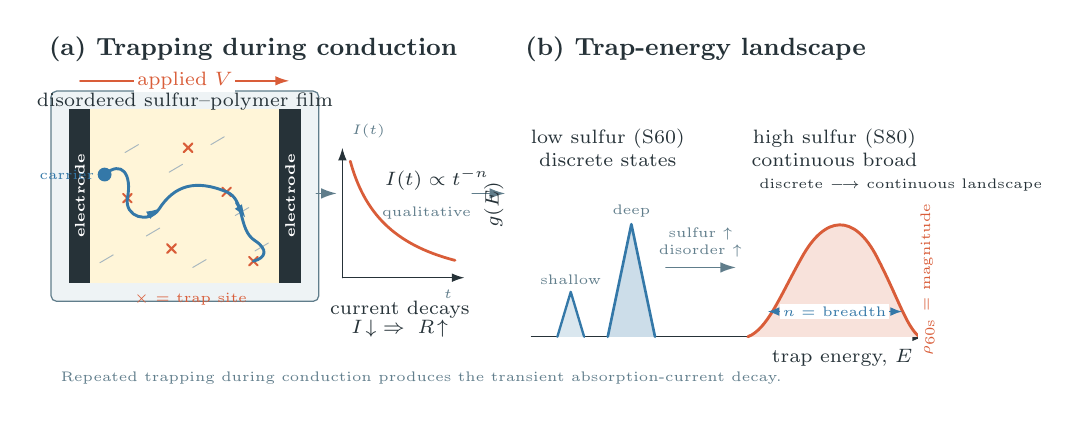
\begin{tikzpicture}[
  x=1cm,y=1cm,
  line cap=round,line join=round,
  >={Latex[length=2.1mm,width=1.4mm]},
  label/.style={font=\scriptsize, text=ink},
  small/.style={font=\tiny, text=muted},
  axis/.style={draw=ink, line width=.45pt, -{Latex[length=1.6mm,width=1.1mm]}},
  flow/.style={draw=muted, line width=.65pt, -{Latex[length=2mm,width=1.35mm]}},
  trap/.style={draw=accent, line width=.75pt}
]

% panel titles
\node[font=\bfseries\small,text=ink,anchor=west] at (0,4.45) {(a) Trapping during conduction};
\node[font=\bfseries\small,text=ink,anchor=west] at (6.05,4.45) {(b) Trap-energy landscape};

% applied-bias cell
\draw[rounded corners=2pt,fill=pale,draw=muted,line width=.45pt] (.15,1.25) rectangle (3.55,3.92);
\fill[ink] (.38,1.48) rectangle (.65,3.69);
\fill[ink] (3.05,1.48) rectangle (3.32,3.69);
\fill[filmlight] (.65,1.48) rectangle (3.05,3.69);
\node[rotate=90,font=\tiny\bfseries,text=white] at (.515,2.59) {electrode};
\node[rotate=90,font=\tiny\bfseries,text=white] at (3.185,2.59) {electrode};
\node[label,anchor=south] at (1.85,3.55) {disordered sulfur--polymer film};

% disorder texture and chemically agnostic traps
\foreach \x/\y in {.86/1.78,1.18/3.18,1.45/2.12,1.74/2.93,2.04/1.72,2.27/3.28,2.58/2.38,2.83/1.93}{
  \draw[muted!55,line width=.35pt] (\x-.09,\y-.04) -- (\x+.08,\y+.06);
}
\foreach \x/\y in {1.12/2.56,1.68/1.92,1.89/3.20,2.38/2.64,2.72/1.76}{
  \draw[trap] (\x-.055,\y-.055)--(\x+.055,\y+.055) (\x-.055,\y+.055)--(\x+.055,\y-.055);
}

% sign-agnostic tortuous multiple-trapping walk
\draw[blue,line width=1.05pt]
  (.83,2.86) .. controls (1.05,3.05) and (1.18,2.86) .. (1.12,2.56)
  .. controls (1.08,2.32) and (1.39,2.23) .. (1.52,2.42)
  .. controls (1.72,2.73) and (1.99,2.80) .. (2.38,2.64)
  .. controls (2.62,2.54) and (2.52,2.16) .. (2.74,2.02)
  .. controls (2.91,1.91) and (2.88,1.80) .. (2.72,1.76);
\draw[blue,-{Latex[length=1.7mm,width=1.1mm]},line width=.75pt] (1.38,2.34)--(1.53,2.43);
\draw[blue,-{Latex[length=1.7mm,width=1.1mm]},line width=.75pt] (2.50,2.50)--(2.62,2.31);
\fill[blue] (.83,2.86) circle (2.5pt);
\node[small,blue,anchor=east] at (.82,2.86) {carrier};
\node[small,accent,anchor=north] at (1.92,1.48) {$\times$ = trap site};

% voltage cue
\draw[accent,line width=.75pt,-{Latex[length=1.8mm,width=1.2mm]}] (.52,4.05)--(3.18,4.05);
\node[label,accent,fill=white,inner sep=1pt] at (1.85,4.05) {applied $V$};

% qualitative transient-current inset
\begin{scope}[shift={(3.85,1.55)}]
  \draw[axis] (0,0)--(1.55,0) node[small,below left=1pt] {$t$};
  \draw[axis] (0,0)--(0,1.65) node[small,above right=0pt] {$I(t)$};
  \draw[accent,line width=1pt] (.10,1.48) .. controls (.28,.82) and (.66,.42) .. (1.43,.22);
  \node[label,anchor=west] at (.42,1.25) {$I(t)\propto t^{-n}$};
  \node[small,anchor=west] at (.38,.82) {qualitative};
\end{scope}
\node[label,align=center,text=ink] at (4.58,1.02) {current decays\\[-1pt]$I\!\downarrow\;\Rightarrow\;R\!\uparrow$};
\draw[flow] (3.52,2.62)--(3.78,2.62);

% cross-panel bridge
\draw[flow] (5.50,2.62)--(5.92,2.62);

% panel B local coordinate frame
\begin{scope}[shift={(6.20,.65)}]
  % shared energy direction
  \draw[axis] (.05,.15)--(5.05,.15) node[label,below left=1pt] {trap energy, $E$};
  \node[label,rotate=90,anchor=south] at (-.18,1.83) {$g(E)$};

  % low-sulfur discrete distribution: a minor shallow state and dominant deep state
  \fill[blue!18] (.38,.15) -- (.72,.15) -- (.55,.72) -- cycle;
  \draw[blue,line width=.85pt] (.38,.15)--(.55,.72)--(.72,.15);
  \fill[blue!25] (1.02,.15) -- (1.62,.15) -- (1.32,1.58) -- cycle;
  \draw[blue,line width=.95pt] (1.02,.15)--(1.32,1.58)--(1.62,.15);
  \node[label,align=center] at (1.02,2.55) {low sulfur (S60)\\discrete states};
  \node[small] at (.55,.88) {shallow};
  \node[small] at (1.32,1.75) {deep};

  % composition/disorder evolution arrow
  \draw[flow] (1.76,1.03)--(2.65,1.03);
  \node[small,align=center] at (2.20,1.35) {sulfur $\uparrow$\\disorder $\uparrow$};

  % high-sulfur broad continuous distribution
  \path[fill=accent!18]
    (2.80,.15) .. controls (3.05,.25) and (3.20,.65) .. (3.48,1.15)
    .. controls (3.78,1.70) and (4.15,1.72) .. (4.44,1.16)
    .. controls (4.70,.66) and (4.82,.26) .. (4.98,.15) -- cycle;
  \draw[accent,line width=1.05pt]
    (2.80,.15) .. controls (3.05,.25) and (3.20,.65) .. (3.48,1.15)
    .. controls (3.78,1.70) and (4.15,1.72) .. (4.44,1.16)
    .. controls (4.70,.66) and (4.82,.26) .. (4.98,.15);
  \node[label,align=center] at (3.90,2.55) {high sulfur (S80)\\continuous broad};

  % independent breadth and magnitude cues
  \draw[blue,{Latex[length=1.5mm]}-{Latex[length=1.5mm]},line width=.65pt]
    (3.05,.47)--(4.76,.47);
  \node[small,blue,fill=white,inner sep=1pt] at (3.90,.47) {$n$ = breadth};
  \draw[accent,{Latex[length=1.5mm]}-{Latex[length=1.5mm]},line width=.65pt]
    (5.08,.17)--(5.08,1.57);
  \node[small,accent,rotate=90,fill=white,inner sep=1pt] at (5.08,.87) {$\rho_{60\mathrm{s}}$ = magnitude};

  \node[small,anchor=west,text=ink] at (2.82,2.08) {discrete $\longrightarrow$ continuous landscape};
\end{scope}

% compact explanatory footer
\node[small,anchor=west,text=muted] at (.15,.28)
  {Repeated trapping during conduction produces the transient absorption-current decay.};

\end{tikzpicture}
\end{document}
